% Section 9: Jordan Canonical Form  (original handwritten pages 64--76)
% ===== Page 64 =====
\section{Jordan Canonical Form}\label{sec:jordan}
\syllabusweek{Weeks 11--12 --- Jordan canonical forms}
\subsection{Generalized Eigenspaces and the Jordan Form}\label{ss:gen-eigenspaces}
\begin{theorem}[Null-space decomposition]
\leavevmode\origpage{64}%
\[ d(s)=(s-\lambda_1)^{r_1}(s-\lambda_2)^{r_2}\cdots(s-\lambda_k)^{r_k} \]
\[
\C^n=\overbrace{\Null\big((A-\lambda_1I)^{m_1}\big)}^{\dim=r_1}\oplus\overbrace{\Null\big((A-\lambda_2I)^{m_2}\big)}^{\dim=r_2}\oplus\cdots\oplus\overbrace{\Null\big((A-\lambda_kI)^{m_k}\big)}^{\dim=r_k}
\]
\[ m(s)=(s-\lambda_1)^{m_1}(s-\lambda_2)^{m_2}\cdots(s-\lambda_k)^{m_k} \]
\end{theorem}

\point If we form a $P$ matrix out of the columns which are the basis vectors for the null spaces $\Null\big((A-\lambda_iI)^{m_i}\big)$ then we can have
\begin{align*}
\bar A&=P^{-1}AP,\\
P&=\big[\,P_1\mid P_2\mid\dots\mid P_k\,\big]_{n\times n},\\
P_i&=\big[\,\underbrace{b_1^i\;\; b_2^i\;\;\dots\;\; b_{r_i}^i}_{\substack{\text{basis vectors for}\\ \Null((A-\lambda_iI)^{m_i})}}\,\big]_{n\times r_i}
\end{align*}
\explain{$P$ has $r_1+r_2+\dots+r_k=n$ columns.}
\[
\bar A=\begin{bmatrix}\bar A_1 & & & 0\\ & \bar A_2 & & \\ & & \ddots & \\ 0 & & & \bar A_k\end{bmatrix}_{n\times n}
\]
where the size of $\bar A_i$ is $r_i\times r_i$.

\point If $P_i$ is selected in a specific way, we can have
\[
\bar A_i=\begin{bmatrix}\lambda_i & \ast & & 0\\ & \lambda_i & \ast & \\ & & \ddots & \ast\\ 0 & & & \lambda_i\end{bmatrix}_{r_i\times r_i},
\qquad\qquad \ast\in\{0,1\}
\]
In this case $\bar A$ is called the \term{Jordan Canonical Form} (JCF) of $A$.
\begin{insight}[Why $\bar A$ is block diagonal]
Each subspace $\Null\big((A-\lambda_iI)^{m_i}\big)$ is invariant under $A$: if $(A-\lambda_iI)^{m_i}x=0$ then, since $A$ commutes with $(A-\lambda_iI)^{m_i}$, also $(A-\lambda_iI)^{m_i}(Ax)=A(A-\lambda_iI)^{m_i}x=0$. So $A$ maps the columns of $P_i$ into the span of the columns of $P_i$, and in the basis given by the columns of $P$ the matrix $\bar A=P^{-1}AP$ has no entries coupling different blocks. Each $\bar A_i$ has the single eigenvalue $\lambda_i$ (with multiplicity $r_i$). The ``specific way'' of choosing $P_i$ is via Jordan chains $x,\ (A-\lambda_iI)x,\ (A-\lambda_iI)^2x,\dots$; every chain produces one Jordan block (a $\lambda_i$-diagonal with $1$'s above it).
\end{insight}

\begin{example}
\[
A=\bmat{1&0&0\\0&2&1\\0&0&2},\qquad
\left.\begin{aligned}d(s)&=(s-1)(s-2)^2\\ m(s)&=(s-1)(s-2)^2\end{aligned}\right\}\ \text{found before}
\]
\[
\C^3=\underbrace{\Null\big((A-I)\big)}_{\dim=1}\oplus\underbrace{\Null\big((A-2I)^2\big)}_{\dim=2}
\]
\paragraph{Powers of $A-I$.}
\begin{align*}
(A-I)&=\bmat{0&0&0\\0&1&1\\0&0&1}, \quad \rank=2, & \dim\Null(A-I)&=1, & \Null(A-I)&=\Span\left\{\bmat{1\\0\\0}\right\}\\
(A-I)^2&=\bmat{0&0&0\\0&1&2\\0&0&1}, \quad \rank=2, & \dim\Null\big((A-I)^2\big)&=1, & \Null\big((A-I)^2\big)&=\Span\left\{\bmat{1\\0\\0}\right\}\\
&\ \ \vdots\\
(A-I)^l&=\bmat{0&0&0\\0&1&l\\0&0&1}, \quad \rank=2, & \dim\Null\big((A-I)^l\big)&=1, & \Null\big((A-I)^l\big)&=\Span\left\{\bmat{1\\0\\0}\right\}
\end{align*}
\[
\Null(A-I)=\Null\big((A-I)^2\big)=\dots=\Null\big((A-I)^l\big)
\]

% ===== Page 65 =====
\paragraph{Powers of $A-2I$.}\origpage{65}
\begin{align*}
(A-2I)&=\bmat{-1&0&0\\0&0&1\\0&0&0}, & \dim\Null(A-2I)&=1, & \Null(A-2I)&=\Span\left\{\bmat{0\\1\\0}\right\}\\
(A-2I)^2&=\bmat{1&0&0\\0&0&0\\0&0&0}, & \dim\Null\big((A-2I)^2\big)&=2, & \Null\big((A-2I)^2\big)&=\Span\left\{\bmat{0\\1\\0},\bmat{0\\0\\1}\right\}
\end{align*}
\[
\therefore\;\Null(A-2I)\subsetneq\Null\big((A-2I)^2\big)\ \text{(proper subset)}\ =\Null\big((A-2I)^3\big)\cdots
\]
\explain{$\subsetneq$\,: $\subset$ \& $\neq$, i.e.\ subset and not equal.}
\begin{align*}
(A-2I)^3&=\bmat{-1&0&0\\0&0&0\\0&0&0}, & \dim\Null\big((A-2I)^3\big)&=2, & \Null\big((A-2I)^3\big)&=\Span\left\{\bmat{0\\1\\0},\bmat{0\\0\\1}\right\}
\end{align*}
% corrected: notes had N((A-2I)) in the last column; (A-2I)^3 is meant

\sep
In general:
\[\setlength{\arraycolsep}{3pt}
\begin{array}{ccccccccc}
\dim & < & \dim & < \cdots < & \dim & = & \dim & = & \cdots\\
\Null(A-\lambda_iI) & \subsetneq & \Null\big((A-\lambda_iI)^2\big) & \subsetneq\cdots\subsetneq & \underbrace{\Null\big((A-\lambda_iI)^{m_i}\big)}_{\dim=r_i} & = & \Null\big((A-\lambda_iI)^{m_i+1}\big) & = & \cdots
\end{array}
\]
\explain{$\dim=r_i$: largest dimension $\hookrightarrow$ exponent $r_i$ in the characteristic polynomial.}
\end{example}

\begin{example}
\[
A=\left[\begin{array}{ccc|c}1&0&0&0\\0&1&1&0\\0&0&1&0\\\hline 0&0&0&2\end{array}\right],
\qquad
\begin{aligned}
d(s)&=(s-1)^3(s-2)\\
m(s)&=\,?\quad\text{3 possibilities:}
\end{aligned}
\]
\begin{enumerate}[label=\arabic*)]
\item $(s-1)(s-2)$
\item $(s-1)^2(s-2)$\quad $\Leftarrow$ This is the minimal polynomial
\item $(s-1)^3(s-2)$
\end{enumerate}
\begin{align*}
(A-I)&=\bmat{0&0&0&0\\0&0&1&0\\0&0&0&0\\0&0&0&1}, & \dim\Null(A-I)&=2\\
(A-I)^2&=\bmat{0&0&0&0\\0&0&0&0\\0&0&0&0\\0&0&0&1}, & \dim\Null\big((A-I)^2\big)&=3\ \checkmark
\end{align*}
\explain{$\dim\Null\big((A-I)^2\big)=3=r_1$ is reached at power $2$, so $m_1=2$; for $\lambda_2=2$, $r_2=1$ forces $m_2=1$. Hence $m(s)=(s-1)^2(s-2)$; indeed $(A-I)^2(A-2I)=0$ but $(A-I)(A-2I)\neq0$.}
\end{example}

% ===== Page 66 =====
\subsection{Chains of Null Spaces}\label{ss:nullspace-chains}
\origpage{66}%
\point Let $\Sigma_i \triangleq A-\lambda_iI$. Then
\[
\begin{array}{ccccccccccc}
\Null(\Sigma_i) & \subsetneq & \Null(\Sigma_i^2) & \subsetneq & \Null(\Sigma_i^3) & \cdots & \subsetneq & \Null(\Sigma_i^{m_i}) & = & \Null(\Sigma_i^{m_i+1}) & \cdots\\
1\le\dim & < & \dim & < & \dim & \cdots & < & \dim=r_i & = & \dim=r_i &
\end{array}
\]

\begin{proof}
\begin{claim}
$\Null(\Sigma_i^l)\subset\Null(\Sigma_i^{l+1})$
\end{claim}
\begin{minipage}{0.3\textwidth}
\centering
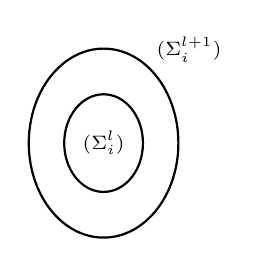
\begin{tikzpicture}
\draw[thick] (0,0) ellipse (0.95 and 1.2);
\draw[thick] (0,0) ellipse (0.5 and 0.62);
\node at (0,0) {\scriptsize $\Null(\Sigma_i^l)$};
\node[anchor=south west] at (0.55,0.9) {\scriptsize $\Null(\Sigma_i^{l+1})$};
\end{tikzpicture}
\end{minipage}\hfill
\begin{minipage}{0.65\textwidth}
\begin{align*}
x\in\Null(\Sigma_i^l)&\Rightarrow \Sigma_i^lx=0\\
&\Rightarrow \Sigma_i\cdot\Sigma_i^lx=\Sigma_i\cdot 0=0\\
&\Rightarrow \Sigma_i^{l+1}x=0\Rightarrow x\in\Null(\Sigma_i^{l+1})
\end{align*}
\end{minipage}

\begin{claim}
If $\Null(\Sigma_i^l)=\Null(\Sigma_i^{l+1})$ then $\Null(\Sigma_i^{l+1})=\Null(\Sigma_i^{l+2})$
% corrected: notes omitted "=" between the two null spaces
\end{claim}
Assume $\Null(\Sigma_i^l)=\Null(\Sigma_i^{l+1})$. Need to show $\Null(\Sigma_i^{l+1})=\Null(\Sigma_i^{l+2})$, i.e.
\begin{enumerate}[label=(\roman*),itemsep=2pt,topsep=2pt]
\item $\Null(\Sigma_i^{l+1})\subset\Null(\Sigma_i^{l+2})$ \quad $\checkmark$ (first claim)
\item $\Null(\Sigma_i^{l+2})\subset\Null(\Sigma_i^{l+1})$
\end{enumerate}
\begin{align*}
x\in\Null(\Sigma_i^{l+2})&\Rightarrow\Sigma_i^{l+2}x=0\\
&\Rightarrow \Sigma_i^{l+1}\,\Sigma_ix=0\Rightarrow\Sigma_ix\in\Null(\Sigma_i^{l+1})\\
&\Rightarrow\Sigma_ix\in\Null(\Sigma_i^l)\\
&\Rightarrow \Sigma_i^l\,\Sigma_ix=0\Rightarrow\Sigma_i^{l+1}x=0\Rightarrow x\in\Null(\Sigma_i^{l+1}) \qedhere
\end{align*}
\end{proof}
\begin{insight}[Consequence]
By the two claims the chain of null spaces grows strictly as long as it grows at all; once two consecutive null spaces coincide it is constant forever. Since the dimensions are bounded by $n$, the chain must stop growing, and it \key{stops exactly at the power $m_i$} (the exponent in $m(s)$), where the dimension equals the algebraic multiplicity $r_i$. Because each step adds at least one dimension, $m_i\le r_i$ again.
\end{insight}

\begin{example}
\[
A=\begin{bmatrix}
\boxed{\begin{smallmatrix}2&1&0\\0&2&1\\0&0&2\end{smallmatrix}} & & & & & \\
& \boxed{\begin{smallmatrix}2&1\\0&2\end{smallmatrix}} & & & & \\
& & \boxed{2} & & & \\
& & & \boxed{2} & & \\
& & & & \boxed{\begin{smallmatrix}3&1\\0&3\end{smallmatrix}} & \\
& & & & & \boxed{3}
\end{bmatrix}_{10\times10},
\qquad
\begin{aligned}
&\dim\Null\big((A-\lambda_iI)^l\big)=\,?\\
&d(s)=\,?\\
&m(s)=\,?
\end{aligned}
\]
\explain{Block diagonal; all entries outside the boxed blocks are zero.}

\paragraph{First block.}
\[
A_1=\bmat{2&1&0\\0&2&1\\0&0&2},\qquad d_1(s)=(s-2)^3,\qquad m_1(s)=(s-2)^3
\]
\begin{align*}
A_1-2I&=\bmat{0&1&0\\0&0&1\\0&0&0},\quad \rank=2, & \dim\Null(A_1-2I)&=1\\
(A_1-2I)^2&=\bmat{0&0&1\\0&0&0\\0&0&0}, & \dim\Null\big((A_1-2I)^2\big)&=2\\
(A_1-2I)^3&=\bmat{0&0&0\\0&0&0\\0&0&0}, & \dim\Null\big((A_1-2I)^3\big)&=3\\
(A_1-2I)^4&=0_{3\times3}, & \dim\Null\big((A_1-2I)^4\big)&=3\ \dots
\end{align*}
\explain{For $(A_1-2I)^3$: no need to calculate as it can be max 3 and is not equal to 1 or 2.}
% corrected: notes write "A" instead of "A_1" in the dimension column and in the last row
\explain{Each Jordan block of size $p$ behaves the same way: $\dim\Null\big((J-\lambda I)^l\big)=\min(l,p)$. Each block of $A$ contributes to the dimensions of $A$ independently.}

% ===== Page 67 =====
\needspace{14\baselineskip}
\paragraph{Whole matrix $A$.}\origpage{67}
\[
d(s)=(s-2)^7(s-3)^3
\]
\explain{$\lambda=2$ appears in blocks of sizes $3,2,1,1$ ($3+2+1+1=7$); $\lambda=3$ in blocks of sizes $2,1$ ($2+1=3$).}
\begin{align*}
&\Sigma_1=A-2I & &\Sigma_2=A-3I\\
&\dim\Null(\Sigma_1)=4 & &\dim\Null(\Sigma_2)=2\\
&\dim\Null(\Sigma_1^2)=6 \quad(+2) & &\dim\Null(\Sigma_2^2)=3 \quad(+1)\\
&\dim\Null(\Sigma_1^3)=7 \quad(+1) & &\Rightarrow (s-3)^2 \quad(+0)\\
&\Rightarrow (s-2)^3 \quad(+0)
\end{align*}
\[
\boxed{\therefore\ m(s)=(s-2)^{3}(s-3)^{2}}
\]
\explain{Exponent 3: largest Jordan block (JB) for $\lambda_i=2$;\quad exponent 2: largest JB for $\lambda_i=3$.}
\end{example}

\subsection{Counting Jordan Blocks}\label{ss:counting-jb}
\begin{align*}
\dim\Null(\Sigma_i)&=\#\text{ of JB's for }\lambda_i\\
&=\#\text{ of JB's with size}\ge1\text{ for }\lambda_i\\
&=\max\#\text{ of linearly independent eigenvectors for }\lambda_i
\end{align*}
\begin{align*}
\dim\Null(\Sigma_i^2)-\dim\Null(\Sigma_i^1)&=\#\text{ of JB's with size}\ge2\text{ for }\lambda_i\\
\dim\Null(\Sigma_i^3)-\dim\Null(\Sigma_i^2)&=\#\text{ of JB's with size}\ge3\text{ for }\lambda_i\\
&\;\;\vdots\\
\dim\Null(\Sigma_i^{l})-\dim\Null(\Sigma_i^{l-1})&=\#\text{ of JB's with size}\ge l\text{ for }\lambda_i.
\end{align*}
% corrected: notes had dim N(Sigma^{l+1}) - dim N(Sigma^l) = # JB's with size >= l (off by one);
% shifted indices so that the case l=1 below is the first line
\paragraph{For $l=1$.}
\[
\dim\Null(\Sigma_i)-\underbrace{\dim\Null\big(\overbrace{\Sigma_i^0}^{I}\big)}_{0}=\#\text{ of JB's with size}\ge1\text{ for }\lambda_i
\]
\explain{Works for $l=1$ also.}

\key{$m_i$ is the size of the largest JB.}
\begin{insight}[Reading off the block sizes]
Write $\delta_l=\dim\Null(\Sigma_i^l)-\dim\Null(\Sigma_i^{l-1})$ (the increments, $\delta_l=\#$ JB's of size $\ge l$). Then
\[
\#\text{ of JB's of size exactly } l \;=\; \delta_l-\delta_{l+1}.
\]
Reason: a block of size $p$ contributes $1$ to $\dim\Null(\Sigma_i^l)$ for each $l\le p$, so it raises the dimension by one at each of the steps $l=1,\dots,p$ and not after. The increments therefore stop being positive at $l=m_i$, the size of the largest block.
\end{insight}

\sep
\needspace{10\baselineskip}
\point For diagonalizable matrix, minimal polynomial should have the power at most 1:
\begin{keybox}
\centering JCF is diagonal iff $m_i=1\ \forall i$
\end{keybox}
\begin{align*}
\C^n&=\Null(\Sigma_1^{m_1})\oplus\cdots\oplus\Null(\Sigma_k^{m_k})\\
\C^n&=\underbrace{\Null(\Sigma_1)}_{r_1}\oplus\cdots\oplus\underbrace{\Null(\Sigma_k)}_{r_k}
\end{align*}
\explain{$\Null(\Sigma_1)$: at most $r_1$ linearly independent eigenvectors.}
The second decomposition holds exactly when $m_i=1$ for all $i$, i.e.\ when $\dim\Null(\Sigma_i)=r_i$ for every eigenvalue.

Hence \key{$A$ is diagonalizable iff there exist $n$ linearly independent eigenvectors for $A$.}

% ===== Page 68 =====
\begin{example}
\leavevmode\origpage{68}\[
A=\bmat{1&-1&1&0\\1&-1&0&0\\0&0&0&0\\2&-2&-2&0}
\quad\Rightarrow\quad
\begin{aligned}
&d(s)=s^4\\
&m(s)=\,?\\
&\text{JCF}=\,?
\end{aligned}
\]
\explain{$d(s)=s^4$: Learn to calculate this! (Shortcut: $A^3=0$ below, so every eigenvalue satisfies $\lambda^3=0$, i.e.\ $\lambda=0$ with multiplicity 4.)}
\begin{align*}
\Sigma_1&=A-\cancel{\lambda_1}^{\,0}I=A, &
\dim\Null(\Sigma_1)&=2, \quad \dim\Null(\Sigma_1^2)=3, \quad \dim\Null(\Sigma_1^3)=4
\end{align*}
\[
A^2=\bmat{0&0&1&0\\0&0&1&0\\0&0&0&0\\0&0&2&0},\qquad
A^3=\bmat{0&0&0&0\\0&0&0&0\\0&0&0&0\\0&0&0&0}
\]
\explain{$\rank A=2$ (row 4 $=-2\cdot$row 1$+4\cdot$row 2, row 3 $=0$) $\Rightarrow\dim\Null(A)=2$; $\rank A^2=1\Rightarrow\dim\Null(A^2)=3$; $A^3=0\Rightarrow\dim\Null(A^3)=4$.}
\begin{align*}
&\therefore\ m(s)=s^3\\
&\#\text{ of JB's}=2 &&(2-0)\\
&\#\text{ of JB's with size}\ge2=1 &&(3-2)\\
&\#\text{ of JB's with size}\ge3=1 &&(4-3)\\
&\#\text{ of JB's with size}\ge4=0 &&(4-4)
\end{align*}
Hence one JB with size $=3$, zero JB with size $=2$, one JB with size $=1$:
\[
\text{JCF}=\left[\begin{array}{ccc|c}0&1&0&0\\0&0&1&0\\0&0&0&0\\\hline0&0&0&0\end{array}\right]
\]
Hence \key{not diagonalizable!} Only $\dim\Null(A)=2<4$ independent eigenvectors exist; equivalently, $m_1=3\neq1$.
\end{example}

\needspace{12\baselineskip}
\begin{example}
Let $A\in\R^{8\times8}$ have the following subspace dimensions:
\begin{alignat*}{2}
\dim\Null(A-3I)&=5 &\qquad& (+5)\\
\dim\Null\big((A-3I)^2\big)&=7 && (+2)\\
\dim\Null\big((A-3I)^3\big)&=8 && (+1)\\
& && (+0)
\end{alignat*}
$d(s)=\,?$\quad $m(s)=\,?$\quad $\text{JCF}=\,?$
\begin{align*}
m(s)&=(s-3)^3\\
d(s)&=(s-3)^8
\end{align*}
\explain{$\Rightarrow$ the maximum number of linearly independent eigenvectors is 5.}
\explain{$\dim\Null\big((A-3I)^3\big)=8=n$, so $3$ is the only eigenvalue ($r_1=8$) and the chain stops at power $3$ ($m_1=3$).}
Block sizes from the increments $5,2,1,0$: \ $5$ JB's in total; $5-2=3$ of size $1$, $2-1=1$ of size $2$, $1-0=1$ of size $3$ \ (check: $3\cdot1+1\cdot2+1\cdot3=8$).
\[
\text{JCF}=\left[\begin{array}{ccc|cc|c|c|c}
3&1&0&0&0&0&0&0\\
0&3&1&0&0&0&0&0\\
0&0&3&0&0&0&0&0\\\hline
0&0&0&3&1&0&0&0\\
0&0&0&0&3&0&0&0\\\hline
0&0&0&0&0&3&0&0\\\hline
0&0&0&0&0&0&3&0\\\hline
0&0&0&0&0&0&0&3
\end{array}\right]
\]
\end{example}

\begin{example}
Let $A\in\R^{4\times4}$. Single eigenvalue at $\lambda=7$, $m_1=2$. Find all possible JCFs the matrix $A$ can have.
\begin{align*}
d(s)&=(s-7)^4\\
m(s)&=(s-7)^2
\end{align*}
\[
\begin{array}{ccc}
\Null(A-7I) & \subsetneq & \Null\big((A-7I)^2\big)\\
1\le\ \ ? & & 4\\
\scriptstyle \dim=2\text{ or }3\text{ or }1 & &
\end{array}
\]
% (example continues on page 69 -- closed in part7)

% ============================================================
% PART 7 : original pages 69--80
% ============================================================
% (continues the example opened at the end of part6: A in R^{4x4}, single eigenvalue 7)

% ===== Page 69 =====
\origpage{69}
\paragraph{Case I: $\dim\Null(A-7I)=3$.}
\[
\begin{array}{r@{\quad}ccccccc}
 & \{0\} & \subsetneq & \Null(A-7I) & \subsetneq & \Null(A-7I)^2 & \subsetneq & \cdots\\
\dim: & 0 & & 3 & & 4 & & 4\\
\text{increment:} & & +3 & & +1 & & +0 &\\
 & & \downarrow & & \downarrow & & &\\
 & & \text{\small 2 JB's of size 1} & & \text{\small 1 JB of size 2} & & &
\end{array}
\]
\[
A=\left[\begin{array}{cc|c|c}
7 & 1 & 0 & 0\\
0 & 7 & 0 & 0\\ \hline
0 & 0 & 7 & 0\\ \hline
0 & 0 & 0 & 7
\end{array}\right]
\qquad \text{\textcircled{\small 1} 1st possibility}
\]

\paragraph{Case II: $\dim\Null(A-7I)=2$.}
\[
\begin{array}{r@{\quad}ccccccc}
 & \{0\} & \subsetneq & \Null(A-7I) & \subsetneq & \Null(A-7I)^2 & \subsetneq & \cdots\\
\dim: & 0 & & 2 & & 4 & & 4\\
\text{increment:} & & +2 & & +2 & & +0 &
\end{array}
\]
\[
A=\left[\begin{array}{cc|cc}
7 & 1 & 0 & 0\\
0 & 7 & 0 & 0\\ \hline
0 & 0 & 7 & 1\\
0 & 0 & 0 & 7
\end{array}\right]
\qquad \text{\textcircled{\small 2} 2nd possibility}
\]

\paragraph{Case III: $\dim\Null(A-7I)=1$.}
\[
\begin{array}{r@{\quad}ccccccc}
 & \{0\} & \subsetneq & \Null(A-7I) & \subsetneq & \Null(A-7I)^2 & \subsetneq & \cdots\\
\dim: & 0 & & 1 & & 4 & & 4\\
\text{increment:} & & +1 & & +3 & & +0 &
\end{array}
\]
\explain{These increments must decrease or stay constant $\Rightarrow$ no such matrix $A$ exists!}

$\therefore$ \key{Two possibilities.}

\begin{insight}[Why the increments cannot grow]
The increment $\dim\Null(A-7I)^{k}-\dim\Null(A-7I)^{k-1}$ equals the number of Jordan blocks of size $\geq k$. Every block of size $\geq k+1$ also has size $\geq k$, so the increments form a non-increasing sequence. In Case~III they would be $1,3,0$: there would be one block in total but three blocks of size $\geq2$, which is impossible. Equivalently: with $\dim\Null(A-7I)=1$ there is a single Jordan block, so it must be $4\times4$; then $m(s)=(s-7)^4$ and $\dim\Null(A-7I)^2=2$, not $4$.
\end{insight}
\end{example}

\subsection{Generalized Eigenvectors and Jordan Chains}\label{ss:chains}
Let $x\in\Null(\Sigma_i^{m_i})$, $x\notin\Null(\Sigma_i^{m_i-1})$:
% corrected: notes had "Sigma_i^{m_i-1} != 0" (the vector x was missing)
\[
\Sigma_i^{m_i}x=0, \qquad \Sigma_i^{m_i-1}x\neq 0 \quad\Rightarrow\quad x\text{: \term{generalized eigenvector}}
\]
\[
\{\underbrace{\Sigma_i^{m_i-1}x}_{\text{not zero}},\ \Sigma_i^{m_i-2}x,\ \dots,\ \Sigma_i x,\ x\}
\quad\Rightarrow\quad \text{none of the vectors are equal to zero.}\sidenote{\term{Jordan chain}}
\]
\explain{If $\Sigma_i^{m_i-2}x$ were zero, then $\Sigma_i(\Sigma_i^{m_i-2}x)=\Sigma_i^{m_i-1}x$ would be zero $\Rightarrow$ it cannot be.}

\begin{claim}
The vectors of the Jordan chain are linearly independent.
\end{claim}
\begin{proof}
Suppose
\begin{align*}
&\alpha_1\Sigma_i^{m_i-1}x+\alpha_2\Sigma_i^{m_i-2}x+\dots+\alpha_{m_i-1}\Sigma_i x+\alpha_{m_i}x=0.
\end{align*}
Multiplying by $\Sigma_i^{m_i-1}$:
\begin{align*}
&\alpha_1\underbrace{\cancel{\Sigma_i^{2m_i-2}}}_{0}x+\alpha_2\underbrace{\cancel{\Sigma_i^{2m_i-3}}}_{0}x+\dots+\alpha_{m_i-1}\underbrace{\cancel{\Sigma_i^{m_i}}}_{0}x+\alpha_{m_i}\Sigma_i^{m_i-1}x=0\\
&\Rightarrow\ \alpha_{m_i}\Sigma_i^{m_i-1}x=0\ \Rightarrow\ \alpha_{m_i}=0.
\end{align*}
Multiplying the remaining equation
\begin{align*}
&\alpha_1\Sigma_i^{m_i-1}x+\alpha_2\Sigma_i^{m_i-2}x+\dots+\alpha_{m_i-1}\Sigma_i x=0
\intertext{by $\Sigma_i^{m_i-2}$, every term except the last again contains a power $\geq m_i$ of $\Sigma_i$:}
&\alpha_{m_i-1}\Sigma_i^{m_i-1}x=0\ \Rightarrow\ \alpha_{m_i-1}=0.
\end{align*}
Continuing in this way (multiplying by $\Sigma_i^{m_i-3},\dots,\Sigma_i,I$) gives $\alpha_{m_i-2}=\dots=\alpha_1=0$.
\end{proof}

$\therefore$ \key{All vectors of the chain are linearly independent.}

% ===== Page 70 =====
\origpage{70}Where the chain vectors lie:
\begin{align*}
\Sigma_i(\Sigma_i^{m_i-1}x)&=0 &&\Rightarrow\ \Sigma_i^{m_i-1}x\in\Null(\Sigma_i)\\
\Sigma_i^{m_i-1}(\Sigma_i x)&=0 &&\Rightarrow\ \Sigma_i x\in\Null(\Sigma_i^{m_i-1})\\
\Sigma_i^{m_i-2}\Sigma_i x&=\Sigma_i^{m_i-1}x\neq 0 &&\Rightarrow\ \Sigma_i x\notin\Null(\Sigma_i^{m_i-2})
\end{align*}
\explain{In general $\Sigma_i^{k}x\in\Null(\Sigma_i^{m_i-k})$ but $\Sigma_i^{k}x\notin\Null(\Sigma_i^{m_i-k-1})$: the $k$-th vector of the chain sits exactly in the ``layer'' $\Null(\Sigma_i^{m_i-k})\setminus\Null(\Sigma_i^{m_i-k-1})$.}

\begin{center}
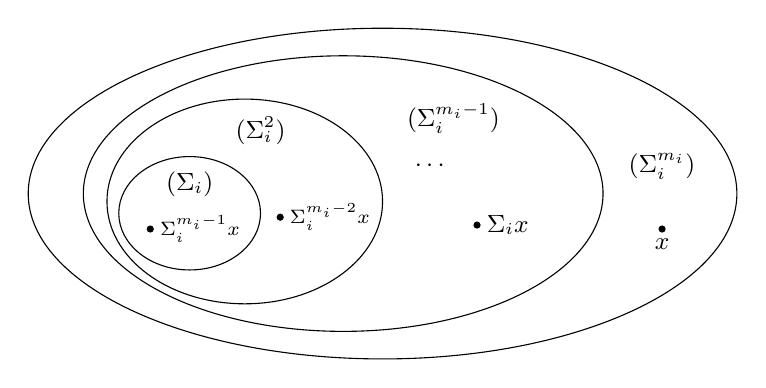
\begin{tikzpicture}[every node/.style={font=\small}]
\draw (0,0) ellipse (4.5 and 2.1);
\draw (-0.5,0) ellipse (3.3 and 1.75);
\draw (-1.75,-0.1) ellipse (1.75 and 1.3);
\draw (-2.45,-0.25) ellipse (0.9 and 0.72);
\node at (-2.45,0.12) {$\Null(\Sigma_i)$};
\fill (-2.95,-0.45) circle (1.3pt) node[right] {\scriptsize $\Sigma_i^{m_i-1}x$};
\node at (-1.55,0.8) {$\Null(\Sigma_i^2)$};
\fill (-1.3,-0.3) circle (1.3pt) node[right] {\scriptsize $\Sigma_i^{m_i-2}x$};
\node at (0.9,0.95) {$\Null(\Sigma_i^{m_i-1})$};
\node at (0.6,0.35) {$\cdots$};
\fill (1.2,-0.4) circle (1.3pt) node[right] {$\Sigma_i x$};
\node at (3.55,0.35) {$\Null(\Sigma_i^{m_i})$};
\fill (3.55,-0.45) circle (1.3pt) node[below] {$x$};
\end{tikzpicture}
\end{center}

\needspace{14\baselineskip}
\subsection{Computing \texorpdfstring{$J$}{J} and \texorpdfstring{$P$}{P}: Worked Examples}\label{ss:jordan-examples}
\begin{example}
\[
A=\bmat{1&1&-1\\-1&3&2\\0&0&1}
\qquad d(s)=?\quad m(s)=?\quad \text{JCF}=?\quad P=?
\]
\[
sI-A=\bmat{s-1&-1&1\\1&s-3&-2\\0&0&s-1}
\]
Expanding along the last row (signs $+\ -\ +$; only the $(3,3)$ entry is nonzero):
\begin{align*}
d(s)=\det(sI-A)&=(s-1)\begin{vmatrix}s-1&-1\\1&s-3\end{vmatrix}\\
&=(s-1)\big[(s-1)(s-3)+1\big]\\
&=(s-1)(s^2-4s+4)\\
\Aboxed{d(s)&=(s-1)(s-2)^2} \qquad \lambda_1=2,\ \ \lambda_2=1
\end{align*}
\[
\Sigma_1=A-2I=\bmat{-1&1&-1\\-1&1&2\\0&0&-1},\qquad \rank=2,\quad \dim\Null(\Sigma_1)=1
\]
$m(s)$ possibilities:
\begin{enumerate}[label=\arabic*),nosep]
\item $(s-1)(s-2)$ \quad $\times$
\item $(s-1)(s-2)^2$ \quad $\checkmark$
\end{enumerate}
\begin{center}
$\dim\Null(\Sigma_1)=1\ \Rightarrow\ \text{not }2\quad\Rightarrow\quad
\boxed{m(s)=(s-1)(s-2)^2}$
\end{center}
\explain{If $m_1=1$, then $\Null(\Sigma_1)=\Null(\Sigma_1^{m_1})$ would have dimension $r_1=2$; but $\dim\Null(\Sigma_1)=3-\rank\Sigma_1=1$, so $m_1=2$.}
Further,
\[
\Sigma_1^2=\bmat{0&0&4\\0&0&1\\0&0&1}
\qquad\qquad
\Sigma_2=A-I=\bmat{0&1&-1\\-1&2&2\\0&0&0},\quad \rank=2,\quad \dim\Null(\Sigma_2)=1
\]
% ===== Page 71 =====
\[
\begin{array}{r@{\quad}ccccc}
 & \Null(\Sigma_1) & \subsetneq & \Null(\Sigma_1^2) & = & \Null(\Sigma_1^3)\\
\dim: & 1 & & 2 & & 2\\
\text{increment:} & +1 & & +1 & & +0
\end{array}
\qquad\qquad
\begin{array}{r@{\quad}ccc}
 & \Null(\Sigma_2) & = & \Null(\Sigma_2^2)\\
\dim: & 1 & & 1
\end{array}
\]
\origpage{71}Hence 1 JB of size 1 for $\lambda_2$.
% corrected: notes had "# of JB w.s.=2 for lambda_2" and "# of JB with size=3 for lambda_2"; these counts are for lambda_1 and mean size >= 2, >= 3
\begin{align*}
(\#\text{ of JB's for }\lambda_1)&=\dim\Null(\Sigma_1)=1\\
(\#\text{ of JB's with size}\geq2\text{ for }\lambda_1)&=\dim\Null(\Sigma_1^2)-\dim\Null(\Sigma_1)=1\\
(\#\text{ of JB's with size}\geq3\text{ for }\lambda_1)&=\dim\Null(\Sigma_1^3)-\dim\Null(\Sigma_1^2)=0
\end{align*}
\explain{Differences of consecutive counts: $1-1=0$ JB of size exactly $1$, \ $1-0=1$ JB of size exactly $2$.}
Hence 1 JB of size 2 for $\lambda_1$:
\[
J=\left[\begin{array}{cc|c}2&1&0\\0&2&0\\\hline 0&0&1\end{array}\right]
\]

\sep
\begin{minipage}[c]{0.32\textwidth}
\centering
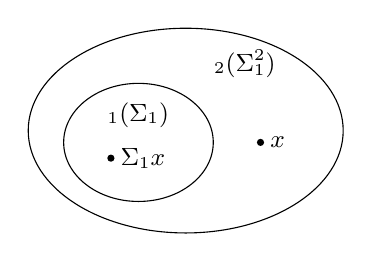
\begin{tikzpicture}[every node/.style={font=\small}]
\draw (0,0) ellipse (2.0 and 1.3);
\draw (-0.6,-0.15) ellipse (0.95 and 0.75);
\node at (0.75,0.85) {$\Null_2(\Sigma_1^2)$};
\node at (-0.6,0.2) {$\Null_1(\Sigma_1)$};
\fill (-0.95,-0.35) circle (1.3pt) node[right] {$\Sigma_1 x$};
\fill (0.95,-0.15) circle (1.3pt) node[right] {$x$};
\end{tikzpicture}
\end{minipage}\hfill
\begin{minipage}[c]{0.64\textwidth}
$x\in\Null(\Sigma_1^2)$, \quad $x\notin\Null(\Sigma_1)$:
\[
x=\bmat{0\\1\\0}\quad\text{or}\quad x=\bmat{1\\0\\0}\quad\cdots
\]
\key{$P$ matrix is not unique}, e.g.:
\begin{align*}
J&=P^{-1}AP, \qquad P_1=2P\\
P_1^{-1}AP_1&=\tfrac12 P^{-1}AP\cdot 2=P^{-1}AP=J
\end{align*}
\end{minipage}

Choosing the first one:
\[
x=\bmat{0\\1\\0},\qquad \Sigma_1x=\bmat{1\\1\\0},\qquad \{\Sigma_1 x, x\}
\]
\begin{itemize}[noitemsep]
\item $x$: generalized eigenvector; \quad \key{$\Sigma_1 x$: should be eigenvector.}
\item $\{\Sigma_1x,x\}$: linearly independent, form a basis for $\Null(\Sigma_1^2)$.
\end{itemize}

\begin{minipage}[c]{0.2\textwidth}
\centering
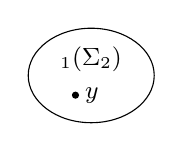
\begin{tikzpicture}[every node/.style={font=\small}]
\draw (0,0) ellipse (0.8 and 0.6);
\node at (0,0.2) {$\Null_1(\Sigma_2)$};
\fill (-0.2,-0.25) circle (1.3pt) node[right] {$y$};
\end{tikzpicture}
\end{minipage}\hfill
\begin{minipage}[c]{0.76\textwidth}
$y\in\Null(\Sigma_2)$, \quad $y\notin\Null(\Sigma_2^0)=\Null(I)=\{0\}$ \quad ($y$ should be nonzero)
\[
y=\bmat{4\\1\\1}
\]
\end{minipage}

\sep
\[
\bar A=P^{-1}AP,\qquad P\bar A=AP,\qquad P=\left[\begin{array}{cc|c}\Sigma_1x & x & y\end{array}\right]
\]
\[
\underbrace{\bmat{1&0&4\\1&1&1\\0&0&1}}_{P}
\underbrace{\left[\begin{array}{cc|c}2&1&0\\0&2&0\\\hline 0&0&1\end{array}\right]}_{\bar A=J}
=A\bmat{1&0&4\\1&1&1\\0&0&1}=\bmat{2&1&4\\2&3&1\\0&0&1}
\]
% note: in the notes the line starts with "P=" labelling the first matrix (the line shows P*Abar = A*P)
\explain{Check: column by column, $PJ=[\,2\Sigma_1x\ \big|\ \Sigma_1x+2x\ \big|\ y\,]$ and $AP=[\,A\Sigma_1x\ |\ Ax\ |\ Ay\,]$ both equal the matrix on the right, and $\det P=1\neq0$, so $P^{-1}AP=J$.}

For $P=\left[\begin{array}{cc|c}x&\Sigma_1x&y\end{array}\right]$:
\[
J=\left[\begin{array}{cc|c}2&0&\\1&2&\\\hline &&1\end{array}\right]
\qquad \times\ \text{not accepted}
\]
\explain{This is also a JCF, but it is not required in this course.}
% ===== Page 72 =====
\origpage{72}Starting the columns of $P$ with $y$ instead:
\begin{align*}
P&=\left[\begin{array}{c|cc}y&\Sigma_1x&x\end{array}\right]: &
\bar A&=\left[\begin{array}{c|cc}1&0&0\\\hline 0&2&1\\0&0&2\end{array}\right]\ \checkmark\\[4pt]
P&=\left[\begin{array}{c|cc}y&x&\Sigma_1x\end{array}\right]: &
\bar A&=\left[\begin{array}{c|cc}1&0&0\\\hline 0&2&0\\0&1&2\end{array}\right]\ \times
\end{align*}
\explain{The second one (crossed out in the notes): this ordering will not be expected in this course.}

\begin{insight}[Recipe used in this example]
\begin{enumerate}[nosep]
\item Factor $d(s)$; for each $\lambda_i$ form $\Sigma_i=A-\lambda_iI$ and compute $\dim\Null(\Sigma_i^k)$, $k=1,2,\dots$ until it reaches $r_i$; the first such $k$ is $m_i$.
\item Increments of these dimensions give the number of JBs of size $\geq k$; their differences give the number of JBs of each size.
\item For each block of size $p$ pick a vector $x\in\Null(\Sigma_i^{p})\setminus\Null(\Sigma_i^{p-1})$ and put the chain $\Sigma_i^{p-1}x,\dots,\Sigma_ix,x$ (eigenvector first) into consecutive columns of $P$, choosing the chains so that all columns are linearly independent.
\end{enumerate}
The ordering \emph{eigenvector first} is what produces the 1's above the diagonal; reversing a chain puts them below the diagonal.
\end{insight}
\end{example}

\subsection{Special Cases}\label{ss:jordan-special}

\paragraph{Case I: $A\in\C^{n\times n}$, single eigenvalue $\lambda_i$.}
We have $m_i=r_i$.
\[
d(s)=(s-\lambda_i)^{r_i},\qquad m(s)=(s-\lambda_i)^{m_i=r_i}=d(s)
\]
\[
\underbrace{\C^n}_{\dim n}=\Null(\Sigma_i^{m_i}),\qquad \dim\Null(\Sigma_i^{m_i})=r_i=n,\qquad n=r_i=m_i
\]
\[
\begin{array}{ccccccccc}
\Null(\Sigma_i) &\subsetneq& \Null(\Sigma_i^2) &\subsetneq& \cdots &\subsetneq& \Null(\Sigma_i^{m_i-1}) &\subsetneq& \Null(\Sigma_i^{m_i})\\
1 &\underbrace{<}_{+1}& 2 &<& \cdots &<& m_i-1 &\underbrace{<}_{+1}& r_i=m_i=n
\end{array}
\]
% corrected: notes had "1 <= 1" under N(Sigma_i) (i.e. dim N(Sigma_i) >= 1 and = 1)
\explain{$n$ dimensions have to be gained in $m_i=n$ strict steps, each of at least $+1$ $\Rightarrow$ every increment is exactly $+1$, in particular $\dim\Null(\Sigma_i)=1$.}
\paragraph{Counting Jordan blocks.}
\begin{align*}
\#\text{ of JB's}&=1\\
\#\text{ of JB's with size}\geq 2&=1\\
\#\text{ of JB's with size}\geq 3&=1\\
&\ \,\vdots\\
\#\text{ of JB's with size}\geq m_i&=1\quad\Rightarrow\ \text{\key{single JB of size $m_i=r_i=n$}}\\
\#\text{ of JB's with size}\geq m_i+1&=0
\end{align*}
\[
\text{JB}=\bmat{\lambda_i&1&&&\\&\lambda_i&1&&0\\&&\lambda_i&\ddots&\\0&&&\ddots&1\\&&&&\lambda_i}_{n\times n}
\qquad\qquad J=P^{-1}AP\ \Rightarrow\ P=?
\]
\begin{center}
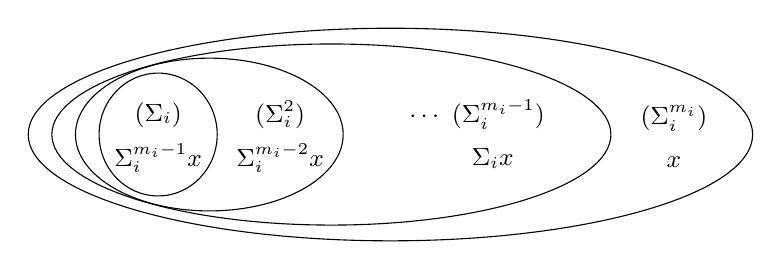
\begin{tikzpicture}[every node/.style={font=\small}]
\draw (0,0) ellipse (4.6 and 1.35);
\draw (-0.75,0) ellipse (3.55 and 1.15);
\draw (-2.3,0) ellipse (1.7 and 0.97);
\draw (-2.95,0) ellipse (0.75 and 0.78);
\node at (-2.95,0.25) {$\Null(\Sigma_i)$};
\node at (-2.95,-0.3) {$\Sigma_i^{m_i-1}x$};
\node at (-1.4,0.25) {$\Null(\Sigma_i^2)$};
\node at (-1.4,-0.3) {$\Sigma_i^{m_i-2}x$};
\node at (1.1,0.25) {$\cdots\ \Null(\Sigma_i^{m_i-1})$};
\node at (1.3,-0.3) {$\Sigma_i x$};
\node at (3.6,0.2) {$\Null(\Sigma_i^{m_i})$};
\node at (3.6,-0.35) {$x$};
\end{tikzpicture}\\[6pt]
$\displaystyle\underbrace{\{\Sigma_i^{m_i-1}x,\ \Sigma_i^{m_i-2}x,\ \dots,\ \Sigma_i x,\ x\}}_{m_i=r_i=n\ \text{linearly independent vectors}}
\qquad \text{1 chain with $n$ elements}$
\end{center}
% ===== Page 73 =====
\noindent\origpage{73}Take the chain as the columns of $P$:
\[
P=\left[\begin{array}{c|c|c|c}\Sigma_i^{m_i-1}x&\cdots&\Sigma_i x&x\end{array}\right],\qquad P\bar A=AP
\]
\begin{align*}
\left[\begin{array}{c|c|c|c}\Sigma_i^{m_i-1}x&\cdots&\Sigma_i x&x\end{array}\right]
\bmat{\lambda_i&1&0&\cdots&0\\0&\lambda_i&1&\cdots&\vdots\\\vdots&0&\lambda_i&\ddots&\vdots\\\vdots&\vdots&0&\ddots&1\\0&0&0&\cdots&\lambda_i}
&=A\left[\begin{array}{c|c|c|c}\Sigma_i^{m_i-1}x&\cdots&\Sigma_i x&x\end{array}\right]\\
&=\left[\begin{array}{c|c|c|c}A\Sigma_i^{m_i-1}x&\cdots&A\Sigma_i x&Ax\end{array}\right]
\end{align*}

\point Since $x\in\Null(\Sigma_i^{m_i})$ \& $x\notin\Null(\Sigma_i^{m_i-1})$:
\begin{align*}
&\Sigma_i^{m_i}x=0,\qquad \Sigma_i^{m_i-1}x\neq 0\\
&\Sigma_i(\Sigma_i^{m_i-1}x)=0\\
&(A-\lambda_iI)(\Sigma_i^{m_i-1}x)=A\Sigma_i^{m_i-1}x-\lambda_i\underbrace{I}_{1}\Sigma_i^{m_i-1}x=0\\
&A\Sigma_i^{m_i-1}x=\lambda_i\Sigma_i^{m_i-1}x
\end{align*}
\point Next vector of the chain:
\begin{align*}
% corrected: notes had "(Sigma_i^{m_i-2}x) Sigma_i" (factor order) and "(lambda_i + Sigma_i)" (lambda_i I + Sigma_i)
&\Sigma_i(\Sigma_i^{m_i-2}x)=\Sigma_i^{m_i-1}x\\
&(A-\lambda_iI)(\Sigma_i^{m_i-2}x)=\Sigma_i^{m_i-1}x\\
&A\Sigma_i^{m_i-2}x=\lambda_i\Sigma_i^{m_i-2}x+\Sigma_i^{m_i-1}x
\end{align*}
\point Similarly:
\begin{align*}
&\Sigma_i(\Sigma_i^{m_i-3}x)=\Sigma_i^{m_i-2}x\\
&(A-\lambda_iI)(\Sigma_i^{m_i-3}x)=\Sigma_i^{m_i-2}x\ \Rightarrow\ A\Sigma_i^{m_i-3}x=\lambda_i\Sigma_i^{m_i-3}x+\Sigma_i^{m_i-2}x
\end{align*}
\explain{Hence column $k$ of $AP$ equals $\lambda_i\cdot(\text{column }k\text{ of }P)+(\text{column }k-1\text{ of }P)$, which is exactly column $k$ of $PJ$: a $\lambda_i$ on the diagonal and a $1$ just above it.}
Altogether:
\[
\{\Sigma_i^{m_i-1}x,\ \Sigma_i^{m_i-2}x,\ \dots,\ \Sigma_i x,\ x\}\quad\text{single chain of size } m_i.
\]

\needspace{10\baselineskip}
\sep
\paragraph{Case II: $A\in\C^{n\times n}$, single eigenvalue $\lambda_i$, $m_i=1$.}
\[
d(s)=(s-\lambda_i)^{r_i},\qquad m(s)=(s-\lambda_i)
\]
\[
\C^n=\underset{r_i=n}{\Null(\Sigma_i^1)}
\qquad\qquad
\begin{array}{ccccc}
\Null(\Sigma_i)&=&\Null(\Sigma_i^2)&=&\cdots\\
r_i&\underbrace{=}_{+0}&r_i&&
\end{array}
\]
\begin{align*}
\#\text{ of JB's}&=r_i=n\\
\#\text{ of JB's with size}\geq 2&=0\quad\Rightarrow\ n\text{ JB's of size }1
\end{align*}
\explain{\key{$m_i$ is the size of the largest JB for $\lambda_i$.}}
% ===== Page 74 =====
\origpage{74}Hence:
\[
J=\bmat{\boxed{\lambda_i}&&&\\&\boxed{\lambda_i}&&\\&&\boxed{\lambda_i}&\\&&&\ddots\ \ \boxed{\lambda_i}}
\]

\begin{minipage}[c]{0.24\textwidth}
\centering
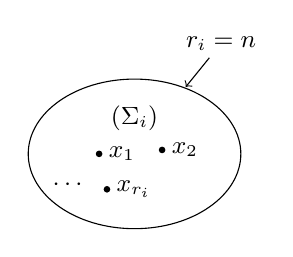
\begin{tikzpicture}[every node/.style={font=\small}]
\draw (0,0) ellipse (1.35 and 0.95);
\node at (1.1,1.4) {$r_i=n$};
\draw[->] (0.95,1.22) -- (0.65,0.85);
\node at (0,0.45) {$\Null(\Sigma_i)$};
\fill (-0.45,0.0) circle (1.2pt) node[right] {$x_1$};
\fill (0.35,0.05) circle (1.2pt) node[right] {$x_2$};
\node at (-0.85,-0.4) {$\cdots$};
\fill (-0.35,-0.45) circle (1.2pt) node[right] {$x_{r_i}$};
\end{tikzpicture}
\end{minipage}\hfill
\begin{minipage}[c]{0.73\textwidth}
$x_1\in\Null(\Sigma_i)$, \quad $x_1\notin\underbrace{\Null(\Sigma_i^0)}_{I}\ \Rightarrow\ x_1\neq 0$: \quad chain $\{x_1\}$\\
$x_2\in\Null(\Sigma_i)$, \quad $x_2\notin\Null(\Sigma_i^0)$: \quad chain $\{x_2\}$\\
\qquad $\Rightarrow$ $x_1$ \& $x_2$ are linearly independent\\
\quad$\vdots$\\
$x_{r_i}\in\Null(\Sigma_i)$, \quad $x_{r_i}\notin\Null(\Sigma_i^0)$: \quad chain $\{x_{r_i}\}$

Hence $r_i=n$ chains of size 1.
\end{minipage}

Each of these vectors is an eigenvector:
\begin{align*}
P&=\left[\begin{array}{c|c|c|c}x_1&x_2&\cdots&x_{r_i}\end{array}\right]\\
P\bar A&=AP\\
\left[\begin{array}{c|c|c|c}x_1&x_2&\cdots&x_{r_i}\end{array}\right]
\underbrace{\bmat{\lambda_i&&0\\&\ddots&\\0&&\lambda_i}}_{\bar A}
&=\left[\begin{array}{cccc}Ax_1&Ax_2&\cdots&Ax_{r_i}\end{array}\right]\\
&=\left[\begin{array}{cccc}\lambda_ix_1&\lambda_ix_2&\cdots&\lambda_ix_{r_i}\end{array}\right]
\quad\text{(as they are eigenvectors)}\\[4pt]
J&=\lambda_iI\\
J&=P^{-1}AP\ \Rightarrow\ A=PJP^{-1}\\
A&=P(\lambda_iI)P^{-1}=\lambda_iPP^{-1}=\lambda_iI
\end{align*}
Equivalently, from the minimal polynomial:
\begin{align*}
m(s)&=s-\lambda_i\\
m(A)&=0_{n\times n}\ \Rightarrow\ A-\lambda_iI=0_{n\times n}\ \Rightarrow\ A=\lambda_iI
\end{align*}

% ===== Page 75 =====
\subsection{Further Examples}\label{ss:jordan-more}
\begin{example}
\leavevmode\origpage{75}$A$ is a $6\times6$ matrix, $\lambda_i$ is the only eigenvalue.
\begin{align*}
d(s)&=(s-\lambda_i)^6, & \dim\Null(\Sigma_i)&=2,\\
m(s)&=(s-\lambda_i)^3, & \dim\Null(\Sigma_i^2)&=4.
\end{align*}
\[
\begin{array}{ccccccc}
\Null(\Sigma_i)&\subsetneq&\Null(\Sigma_i^2)&\subsetneq&\Null(\Sigma_i^3)&=&\Null(\Sigma_i^4)\\
2&&4&&6&&6
\end{array}
\qquad\qquad
\C^6=\Null(\Sigma_i^3)
\]
\begin{itemize}[nosep]
\item $m(s)=(s-\lambda_i)$ would be needed for diagonalizability.
\item At most 2 linearly independent eigenvectors.
\item $\Rightarrow$ \key{not diagonalizable} (it should be 6).
\end{itemize}
\paragraph{Jordan blocks.}
\[
\left.\begin{array}{l}
\#\text{ of JB's}=2\\
\#\text{ of JB's with size}\geq2=2\\
\#\text{ of JB's with size}\geq3=2\\
\#\text{ of JB's with size}\geq4=0
\end{array}\right\}\ \text{2 JB's of size 3}
\qquad
J=\left[\begin{array}{ccc|ccc}
\lambda_i&1&0&&&\\
0&\lambda_i&1&&0&\\
&&\lambda_i&&&\\\hline
&&&\lambda_i&1&0\\
&0&&&\lambda_i&1\\
&&&0&&\lambda_i
\end{array}\right]
\]
\explain{$\#$ of JB's with size $\geq k$ $=\dim\Null(\Sigma_i^k)-\dim\Null(\Sigma_i^{k-1})$: here $2-0$, $4-2$, $6-4$, $6-6$.}

\begin{center}
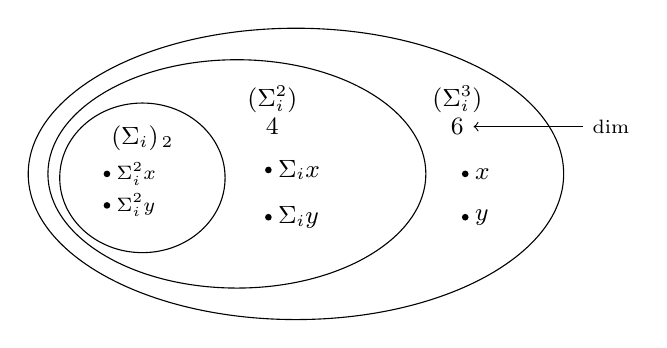
\begin{tikzpicture}[every node/.style={font=\small}]
\draw (0,0) ellipse (3.4 and 1.85);
\draw (-0.75,0) ellipse (2.4 and 1.45);
\draw (-1.95,-0.05) ellipse (1.05 and 0.95);
\node at (-1.95,0.45) {$\Null(\Sigma_i)_{\,2}$};
\fill (-2.4,0.0) circle (1.2pt) node[right] {\scriptsize $\Sigma_i^2x$};
\fill (-2.4,-0.4) circle (1.2pt) node[right] {\scriptsize $\Sigma_i^2y$};
\node at (-0.3,0.95) {$\Null(\Sigma_i^2)$};
\node at (-0.3,0.6) {$4$};
\fill (-0.35,0.05) circle (1.2pt) node[right] {$\Sigma_i x$};
\fill (-0.35,-0.55) circle (1.2pt) node[right] {$\Sigma_i y$};
\node at (2.05,0.95) {$\Null(\Sigma_i^3)$};
\node (six) at (2.05,0.6) {$6$};
\node (dim) at (4.0,0.6) {\scriptsize dim};
\draw[->] (dim.west) -- (six.east);
\fill (2.15,0.0) circle (1.2pt) node[right] {$x$};
\fill (2.15,-0.55) circle (1.2pt) node[right] {$y$};
\end{tikzpicture}
\end{center}
\paragraph{Chains.}
\begin{align*}
&x\in\Null(\Sigma_i^3),\ x\notin\Null(\Sigma_i^2): && \{\Sigma_i^2x,\Sigma_ix,x\}\ \Rightarrow\ \text{alone not sufficient to form a basis}\\
&y\in\Null(\Sigma_i^3),\ y\notin\Null(\Sigma_i^2): && \{\Sigma_i^2y,\Sigma_iy,y\}
\end{align*}
\explain{The two chains together should be linearly independent to form a basis.}

\point Condition: \key{$\Sigma_i^2x$ \& $\Sigma_i^2y$ should be linearly independent.}

\begin{insight}[Why this condition suffices]
Suppose a combination of the six vectors vanishes. Applying $\Sigma_i^2$ kills everything except the coefficients of $x$ and $y$, leaving $a\Sigma_i^2x+b\Sigma_i^2y=0$, so $a=b=0$ by the condition. Applying $\Sigma_i$ to what remains gives the same relation for the coefficients of $\Sigma_ix,\Sigma_iy$, and finally for $\Sigma_i^2x,\Sigma_i^2y$. So independence of the eigenvectors at the bottom of the chains implies independence of the whole set (the same argument as for a single chain).
\end{insight}
\[
P=\left[\begin{array}{ccc|ccc}\Sigma_i^2x&\Sigma_ix&x&\Sigma_i^2y&\Sigma_iy&y\end{array}\right]
\]

\needspace{10\baselineskip}
\sep
\paragraph{Variant.} Continue the same example but with $\dim\Null(\Sigma_i)=3$, $\dim\Null(\Sigma_i^2)=5$.
\[
\begin{aligned}
\#\text{ of JB's}&=3\\
\#\text{ of JB's with size}\geq2&=2\\
\#\text{ of JB's with size}\geq3&=1\\
\#\text{ of JB's with size}\geq4&=0
\end{aligned}
\qquad\Longrightarrow\qquad
\begin{aligned}
&m_i=\text{size of largest JB}=3\\
&1\text{ JB of size }3\\
&1\text{ JB of size }2\\
&1\text{ JB of size }1
\end{aligned}
\]
\[
J=\left[\begin{array}{ccc|cc|c}
\lambda_i&1&0&&&\\
0&\lambda_i&1&&&\\
0&0&\lambda_i&&&\\\hline
&&&\lambda_i&1&\\
&&&0&\lambda_i&\\\hline
&&&&&\lambda_i
\end{array}\right]
\]

\begin{center}
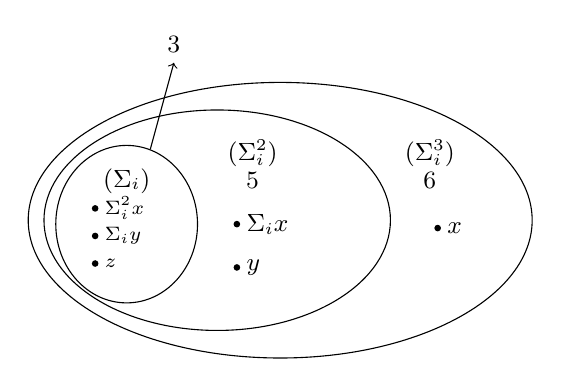
\begin{tikzpicture}[every node/.style={font=\small}]
\draw (0,0) ellipse (3.2 and 1.75);
\draw (-0.8,0) ellipse (2.2 and 1.4);
\draw (-1.95,-0.05) ellipse (0.9 and 1.0);
\node at (-1.95,0.5) {$\Null(\Sigma_i)$};
\draw[->] (-1.65,0.9) -- (-1.35,2.0) node[above] {$3$};
\fill (-2.35,0.15) circle (1.2pt) node[right] {\scriptsize $\Sigma_i^2x$};
\fill (-2.35,-0.2) circle (1.2pt) node[right] {\scriptsize $\Sigma_iy$};
\fill (-2.35,-0.55) circle (1.2pt) node[right] {\scriptsize $z$};
\node at (-0.35,0.85) {$\Null(\Sigma_i^2)$};
\node at (-0.35,0.5) {$5$};
\fill (-0.55,-0.05) circle (1.2pt) node[right] {$\Sigma_ix$};
\fill (-0.55,-0.6) circle (1.2pt) node[right] {$y$};
\node at (1.9,0.85) {$\Null(\Sigma_i^3)$};
\node at (1.9,0.5) {$6$};
\fill (2.0,-0.1) circle (1.2pt) node[right] {$x$};
\end{tikzpicture}
\end{center}
\paragraph{Chains.}
\begin{align*}
&x\in\Null(\Sigma_i^3),\ x\notin\Null(\Sigma_i^2): && \{\Sigma_i^2x,\Sigma_ix,x\}\\
&y\in\Null(\Sigma_i^2),\ y\notin\Null(\Sigma_i): && \{\Sigma_iy,y\}\\
&z\in\Null(\Sigma_i),\ z\notin\Null(\Sigma_i^0)\Rightarrow z\neq0: && \{z\}
\end{align*}
Hence \key{$\Sigma_i^2x,\ \Sigma_iy,\ z$ should be linearly independent.}\origpage{76}
\[
P=\left[\begin{array}{ccc|cc|c}\Sigma_i^2x&\Sigma_ix&x&\Sigma_iy&y&z\end{array}\right]
\]
\end{example}

\begin{example}
\[
A=\bmat{1&1&0&0\\0&1&0&0\\0&0&1&0\\-1&1&0&2}
\qquad
\begin{aligned}
&d(s)=(s-1)^3(s-2),\qquad \lambda_1=1,\ \lambda_2=2\\
&m(s)\,?\quad J\,?\quad P\,?
\end{aligned}
\]
\explain{You should know how to calculate $d(s)$.}
\paragraph{For $\lambda_1=1$.}
\[
\Sigma_1=\bmat{0&1&0&0\\0&0&0&0\\0&0&0&0\\-1&1&0&1},
\quad
\Sigma_1^2=\bmat{0&0&0&0\\0&0&0&0\\0&0&0&0\\-1&0&0&1}
\]
\[
\begin{array}{l}\dim\Null(\Sigma_1)=2,\quad \rank=2\\ \text{it should increase (to }r_1=3)\end{array}
\quad\Rightarrow\quad (s-1)^2(s-2)=m(s)
\]
\[
\begin{array}{ccc}
\Null(\Sigma_1)&\subsetneq&\Null(\Sigma_1^2)\\
2&&3
\end{array}
\ \Rightarrow\
\begin{array}{l}
\text{1 JB of size 2}\\ \text{1 JB of size 1}
\end{array}
\qquad
\begin{array}{ccc}
\Null(\Sigma_2)&=&\Null(\Sigma_2^2)\\
1&&1
\end{array}
\ \Rightarrow\ \text{1 JB of size 1}
\]
\[
\begin{aligned}
\#\text{ of JB's for }\lambda_1&=2\\
\#\text{ of JB's with size}\geq2&=1\\
\#\text{ of JB's with size}\geq3&=0
\end{aligned}
\qquad\qquad
\C^4=\underset{3}{\Null(\Sigma_1^2)}\oplus\underset{1}{\Null(\Sigma_2)}
\qquad
J=\left[\begin{array}{cc|c|c}1&1&&\\0&1&&\\\hline &&1&\\\hline &&&2\end{array}\right]
\]

\begin{minipage}[c]{0.34\textwidth}
\centering
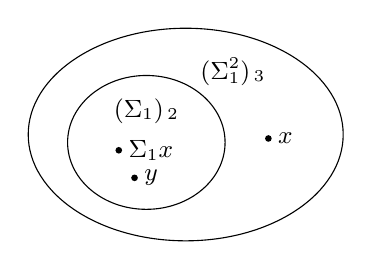
\begin{tikzpicture}[every node/.style={font=\small}]
\draw (0,0) ellipse (2.0 and 1.35);
\draw (-0.5,-0.1) ellipse (1.0 and 0.85);
\node at (0.6,0.8) {$\Null(\Sigma_1^2)_{\,3}$};
\node at (-0.5,0.3) {$\Null(\Sigma_1)_{\,2}$};
\fill (-0.85,-0.2) circle (1.2pt) node[right] {$\Sigma_1x$};
\fill (-0.65,-0.55) circle (1.2pt) node[right] {$y$};
\fill (1.05,-0.05) circle (1.2pt) node[right] {$x$};
\end{tikzpicture}
\end{minipage}\hfill
\begin{minipage}[c]{0.64\textwidth}
$x\in\Null(\Sigma_1^2)$, $x\notin\Null(\Sigma_1)$;\\
$y\in\Null(\Sigma_1)$ \& $y\neq0$;\quad $y$ \& $\Sigma_1x$ linearly independent.
\[
x=\bmat{0\\1\\0\\0},\qquad \Sigma_1x=\bmat{1\\0\\0\\1},\qquad
y=\bmat{0\\0\\1\\0}\ \text{(eigenvector)}
\]
Chains: $\{\Sigma_1x,\ x\}$ and $\{y\}$.
\end{minipage}

\begin{minipage}[c]{0.34\textwidth}
\centering
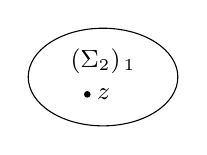
\begin{tikzpicture}[every node/.style={font=\small}]
\draw (0,0) ellipse (0.95 and 0.62);
\node at (0,0.2) {$\Null(\Sigma_2)_{\,1}$};
\fill (-0.2,-0.22) circle (1.2pt) node[right] {$z$};
\end{tikzpicture}
\end{minipage}\hfill
\begin{minipage}[c]{0.64\textwidth}
$z\in\Null(\Sigma_2)$, $z\neq0$:
\[
z=\bmat{0\\0\\0\\1}\qquad\qquad P=\left[\begin{array}{cc|c|c}\Sigma_1x&x&y&z\end{array}\right]
\]
\end{minipage}

\begin{insight}[Check]
\[
P=\bmat{1&0&0&0\\0&1&0&0\\0&0&1&0\\1&0&0&1},\qquad
AP=PJ=\bmat{1&1&0&0\\0&1&0&0\\0&0&1&0\\1&1&0&2},\qquad \det P=1\neq0,
\]
so indeed $P^{-1}AP=J$. ($\Sigma_1^2$ has rank $1$, so $\dim\Null(\Sigma_1^2)=3=r_1$, confirming $m_1=2$.)
\end{insight}
\end{example}
